
 \begin{example}
 We continue the example from above with $P_1=1+p_{1,1}z+p_{1,2}z^2+z^3$ and $P_2=1+p_{2,1}z+z^2$.
 
 For $m=1$, we get $\bfa_1=(1,0)$ so that $D_1=$ 
 \raisebox{0.15em}{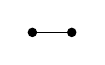
\begin{tikzpicture}
 \begin{scope}[scale=0.5]
 \draw[step=1.0, black, thin] (0,0) grid (1,0);
 \draw[black, thin] (0,0) -- (1,0);
 \draw[black, fill=black] (0,0) circle (3pt);
 \draw[black, fill=black] (1,0) circle (3pt);
 \end{scope}
 \end{tikzpicture}}.
 This maximal Dyck path consists of a single horizontal edge which may be assigned any of the weights $0,1,2,3$, a situation which we denote by the dashed edge
 \raisebox{0.15em}{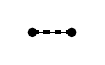
\begin{tikzpicture}
 \begin{scope}[scale=0.5]
 \draw[step=1.0, black, thin] (0,0) grid (1,0);
 \draw[black, thin] (0,0) -- (1,0);
 \draw[black, fill=black] (0,0) circle (3pt);
 \draw[black, line width=1.5pt, dash pattern=on 2.5pt off 1.5pt] (0,0) -- (1,0);
 \draw[black, fill=black] (1,0) circle (3pt);
 \end{scope}
 \end{tikzpicture}}.
 Summing the monomial contributions coming from~\eqref{eq:edge weights} for each choice of weight, we get
 \[Y_{D_1}=X^{-1}+p_{1,1}YX^{-1}+p_{1,2}Y^2X^{-1}+Y^3X^{-1}=Y_1\]
 and this same equality holds for any dashed edge below.

 For $m=2$, we get $\bfa_2=(2,1)$ so that $D_2=$
 \raisebox{-0.5em}{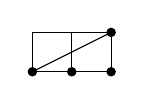
\begin{tikzpicture}
 \begin{scope}[scale=0.5]
 \draw[step=1.0, black, thin] (0,0) grid (2,1);
 \draw[black, thin] (0,0) -- (2,1);
 \draw[black, fill=black] (0,0) circle (3pt);
 \draw[black, fill=black] (1,0) circle (3pt);
 \draw[black, fill=black] (2,0) circle (3pt);
 \draw[black, fill=black] (2,1) circle (3pt);
 \end{scope}
 \end{tikzpicture}}.
 In this case, the compatible weightings of the edges in $D_2$ are given by
 \[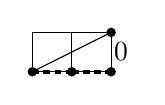
\begin{tikzpicture}
 \begin{scope}[scale=0.5]
 \draw[step=1.0, black, thin] (0,0) grid (2,1);
 \draw[black, thin] (0,0) -- (2,1);
 \draw[black, fill=black] (0,0) circle (3pt);
 \draw[black, line width=1.5pt, dash pattern=on 2.5pt off 1.5pt] (0,0) -- (1,0);
 \draw[black, fill=black] (1,0) circle (3pt);
 \draw[black, line width=1.5pt, dash pattern=on 2.5pt off 1.5pt] (1,0) -- (2,0);
 \draw[black, fill=black] (2,0) circle (3pt);
 \draw[black, fill=black] (2,1) circle (3pt);
 \node at (2.25,0.5) {$0$};
 \end{scope}
 \end{tikzpicture}
 \qquad
 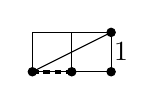
\begin{tikzpicture}
 \begin{scope}[scale=0.5]
 \draw[step=1.0, black, thin] (0,0) grid (2,1);
 \draw[black, thin] (0,0) -- (2,1);
 \draw[black, fill=black] (0,0) circle (3pt);
 \draw[black, line width=1.5pt, dash pattern=on 2.5pt off 1.5pt] (0,0) -- (1,0);
 \draw[black, fill=black] (1,0) circle (3pt);
 \draw[black, fill=black] (2,0) circle (3pt);
 \draw[black, fill=black] (2,1) circle (3pt);
 \node at (2.25,0.5) {$1$};
 \end{scope}
 \end{tikzpicture}
 \qquad
 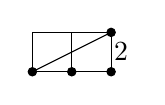
\begin{tikzpicture}
 \begin{scope}[scale=0.5]
 \draw[step=1.0, black, thin] (0,0) grid (2,1);
 \draw[black, thin] (0,0) -- (2,1);
 \draw[black, fill=black] (0,0) circle (3pt);
 \draw[black, fill=black] (1,0) circle (3pt);
 \draw[black, fill=black] (2,0) circle (3pt);
 \draw[black, fill=black] (2,1) circle (3pt);
 \node at (2.25,0.5) {$2$};
 \end{scope}
 \end{tikzpicture}\]
 where we again use a dashed line to indicate that a horizontal edge may be assigned any of the weights $0,1,2,3$ without affecting compatibility.
 Summing the monomial contributions coming from~\eqref{eq:edge weights} for each choice of weight, we get
 \[Y_{D_2}=Y_1^2XY^{-1}X^{-1}+Y_1X^{-1}p_{2,1}X^2Y^{-1}X^{-1}+X^{-1}X^{-1}X^3Y^{-1}X^{-1}=Y_2.\]

 For $m=3$, we get $\bfa_3=(5,3)$ so that $D_3=$
 \raisebox{-1.9em}{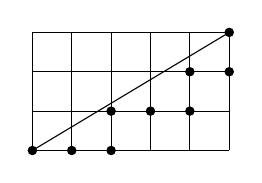
\begin{tikzpicture}
 \begin{scope}[scale=0.5]
 \draw[step=1.0, black, thin] (0,0) grid (5,3);
 \draw[black, thin] (0,0) -- (5,3);
 \draw[black, fill=black] (0,0) circle (3pt);
 \draw[black, fill=black] (1,0) circle (3pt);
 \draw[black, fill=black] (2,0) circle (3pt);
 \draw[black, fill=black] (2,1) circle (3pt);
 \draw[black, fill=black] (3,1) circle (3pt);
 \draw[black, fill=black] (4,1) circle (3pt);
 \draw[black, fill=black] (4,2) circle (3pt);
 \draw[black, fill=black] (5,2) circle (3pt);
 \draw[black, fill=black] (5,3) circle (3pt);
 \end{scope}
 \end{tikzpicture}}.
 In this case, the compatible weightings of the edges in $D_3$ are given by
 \[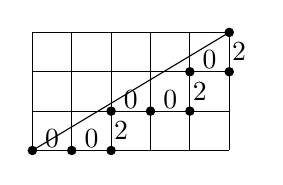
\begin{tikzpicture}
 \begin{scope}[scale=0.5]
 \draw[step=1.0, black, thin] (0,0) grid (5,3);
 \draw[black, thin] (0,0) -- (5,3);
 \draw[black, fill=black] (0,0) circle (3pt);
 \node at (0.5,0.3) {$0$};
 \draw[black, fill=black] (1,0) circle (3pt);
 \node at (1.5,0.3) {$0$};
 \draw[black, fill=black] (2,0) circle (3pt);
 \node at (2.25,0.5) {$2$};
 \draw[black, fill=black] (2,1) circle (3pt);
 \node at (2.5,1.3) {$0$};
 \draw[black, fill=black] (3,1) circle (3pt);
 \node at (3.5,1.3) {$0$};
 \draw[black, fill=black] (4,1) circle (3pt);
 \node at (4.25,1.5) {$2$};
 \draw[black, fill=black] (4,2) circle (3pt);
 \node at (4.5,2.3) {$0$};
 \draw[black, fill=black] (5,2) circle (3pt);
 \node at (5.25,2.5) {$2$};
 \draw[black, fill=black] (5,3) circle (3pt);
 \end{scope}
 \end{tikzpicture}
 \quad
 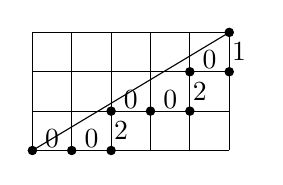
\begin{tikzpicture}
 \begin{scope}[scale=0.5]
 \draw[step=1.0, black, thin] (0,0) grid (5,3);
 \draw[black, thin] (0,0) -- (5,3);
 \draw[black, fill=black] (0,0) circle (3pt);
 \node at (0.5,0.3) {$0$};
 \draw[black, fill=black] (1,0) circle (3pt);
 \node at (1.5,0.3) {$0$};
 \draw[black, fill=black] (2,0) circle (3pt);
 \node at (2.25,0.5) {$2$};
 \draw[black, fill=black] (2,1) circle (3pt);
 \node at (2.5,1.3) {$0$};
 \draw[black, fill=black] (3,1) circle (3pt);
 \node at (3.5,1.3) {$0$};
 \draw[black, fill=black] (4,1) circle (3pt);
 \node at (4.25,1.5) {$2$};
 \draw[black, fill=black] (4,2) circle (3pt);
 \node at (4.5,2.3) {$0$};
 \draw[black, fill=black] (5,2) circle (3pt);
 \node at (5.25,2.5) {$1$};
 \draw[black, fill=black] (5,3) circle (3pt);
 \end{scope}
 \end{tikzpicture}
 \quad
 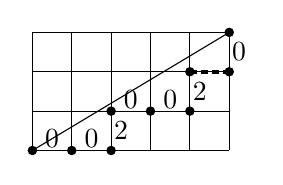
\begin{tikzpicture}
 \begin{scope}[scale=0.5]
 \draw[step=1.0, black, thin] (0,0) grid (5,3);
 \draw[black, thin] (0,0) -- (5,3);
 \draw[black, fill=black] (0,0) circle (3pt);
 \node at (0.5,0.3) {$0$};
 \draw[black, fill=black] (1,0) circle (3pt);
 \node at (1.5,0.3) {$0$};
 \draw[black, fill=black] (2,0) circle (3pt);
 \node at (2.25,0.5) {$2$};
 \draw[black, fill=black] (2,1) circle (3pt);
 \node at (2.5,1.3) {$0$};
 \draw[black, fill=black] (3,1) circle (3pt);
 \node at (3.5,1.3) {$0$};
 \draw[black, fill=black] (4,1) circle (3pt);
 \node at (4.25,1.5) {$2$};
 \draw[black, fill=black] (4,2) circle (3pt);
 \draw[black, line width=1.5pt, dash pattern=on 2.5pt off 1.5pt] (4,2) -- (5,2);
 \draw[black, fill=black] (5,2) circle (3pt);
 \node at (5.25,2.5) {$0$};
 \draw[black, fill=black] (5,3) circle (3pt);
 \end{scope}
 \end{tikzpicture}
 \quad
 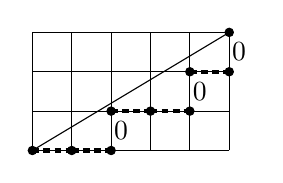
\begin{tikzpicture}
 \begin{scope}[scale=0.5]
 \draw[step=1.0, black, thin] (0,0) grid (5,3);
 \draw[black, thin] (0,0) -- (5,3);
 \draw[black, fill=black] (0,0) circle (3pt);
 \draw[black, line width=1.5pt, dash pattern=on 2.5pt off 1.5pt] (0,0) -- (1,0);
 \draw[black, fill=black] (1,0) circle (3pt);
 \draw[black, line width=1.5pt, dash pattern=on 2.5pt off 1.5pt] (1,0) -- (2,0);
 \draw[black, fill=black] (2,0) circle (3pt);
 \node at (2.25,0.5) {$0$};
 \draw[black, fill=black] (2,1) circle (3pt);
 \draw[black, line width=1.5pt, dash pattern=on 2.5pt off 1.5pt] (2,1) -- (3,1);
 \draw[black, fill=black] (3,1) circle (3pt);
 \draw[black, line width=1.5pt, dash pattern=on 2.5pt off 1.5pt] (3,1) -- (4,1);
 \draw[black, fill=black] (4,1) circle (3pt);
 \node at (4.25,1.5) {$0$};
 \draw[black, fill=black] (4,2) circle (3pt);
 \draw[black, line width=1.5pt, dash pattern=on 2.5pt off 1.5pt] (4,2) -- (5,2);
 \draw[black, fill=black] (5,2) circle (3pt);
 \node at (5.25,2.5) {$0$};
 \draw[black, fill=black] (5,3) circle (3pt);
 \end{scope}
 \end{tikzpicture}
 \]

 To describe the non-commutative generalized cluster variables $Y_1,Y_2,Y_3$ above as pseudo-positive non-commutative Laurent polynomials we consider the following roots and corresponding maximal Dyck paths:
 \[\begin{array}{lccl}
 \raisebox{-0.15em}{$\bfa_1=(1,0)$} & & & \raisebox{-0.15em}{$D_1=$ }
 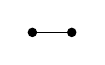
\begin{tikzpicture}
 \begin{scope}[scale=0.5]
 \draw[step=1.0, black, thin] (0,0) grid (1,0);
 \draw[black, thin] (0,0) -- (1,0);
 \draw[black, fill=black] (0,0) circle (3pt);
 \draw[black, fill=black] (1,0) circle (3pt);
 \end{scope}
 \end{tikzpicture}\\
 \raisebox{0.5em}{$\bfa_2=(2,1)$} & & & \raisebox{0.5em}{$D_2=$ }
 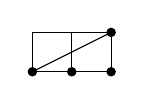
\begin{tikzpicture}
 \begin{scope}[scale=0.5]
 \draw[step=1.0, black, thin] (0,0) grid (2,1);
 \draw[black, thin] (0,0) -- (2,1);
 \draw[black, fill=black] (0,0) circle (3pt);
 \draw[black, fill=black] (1,0) circle (3pt);
 \draw[black, fill=black] (2,0) circle (3pt);
 \draw[black, fill=black] (2,1) circle (3pt);
 \end{scope}
 \end{tikzpicture}\\
 \raisebox{1.9em}{$\bfa_3=(5,3)$} & & & \raisebox{1.9em}{$D_3=$ }
 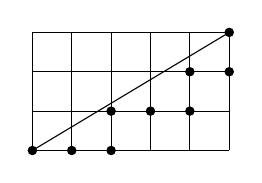
\begin{tikzpicture}
 \begin{scope}[scale=0.5]
 \draw[step=1.0, black, thin] (0,0) grid (5,3);
 \draw[black, thin] (0,0) -- (5,3);
 \draw[black, fill=black] (0,0) circle (3pt);
 \draw[black, fill=black] (1,0) circle (3pt);
 \draw[black, fill=black] (2,0) circle (3pt);
 \draw[black, fill=black] (2,1) circle (3pt);
 \draw[black, fill=black] (3,1) circle (3pt);
 \draw[black, fill=black] (4,1) circle (3pt);
 \draw[black, fill=black] (4,2) circle (3pt);
 \draw[black, fill=black] (5,2) circle (3pt);
 \draw[black, fill=black] (5,3) circle (3pt);
 \end{scope}
 \end{tikzpicture}
 \end{array}\]

 \end{example}
